\documentclass[]{thesis-ekf}
\usepackage[T1]{fontenc}
\PassOptionsToPackage{defaults=hu-min}{magyar.ldf}
\usepackage[magyar]{babel}
\usepackage{mathtools,amssymb,amsthm,pdfpages}
\footnotestyle{rule=fourth}

\newtheorem{tetel}{Tétel}[chapter]
\theoremstyle{definition}
\newtheorem{definicio}[tetel]{Definíció}
\theoremstyle{remark}
\newtheorem{megjegyzes}[tetel]{Megjegyzés}

\begin{document}

\institute{Matematikai és Informatikai Intézet}
\title{PokerParty}
\author{Szabó Márk\\programtervező informatikus Bsc.}
\supervisor{Troll Ede\\tanársegéd}
\city{Eger}
\date{2025}
\maketitle

\tableofcontents

\chapter*{Bevezetés}
\addcontentsline{toc}{chapter}{Bevezetés}

\chapter{Technológiai áttekintés}

\section{Enginek}

\subsection{Unreal}

\subsection{Godot}

\subsection{Unity}

\section{Multiplayer technológia a játékfejlesztésben}

\chapter{Rendszerterv}

\chapter{Saját szoftver megvalósítása}
\section{Multiplayer kapcsolat megvalósítása}
\section{Texas Hold'Em kéz kiértékelés}

\chapter{Tesztelés}

\chapter*{Összegzés}
\addcontentsline{toc}{chapter}{Összegzés}

\begin{thebibliography}{2}
\addcontentsline{toc}{chapter}{\bibname}

\end{thebibliography}

% Aláírt, szkennelt nyilatkozat beillesztése a szakdolgozat végére
%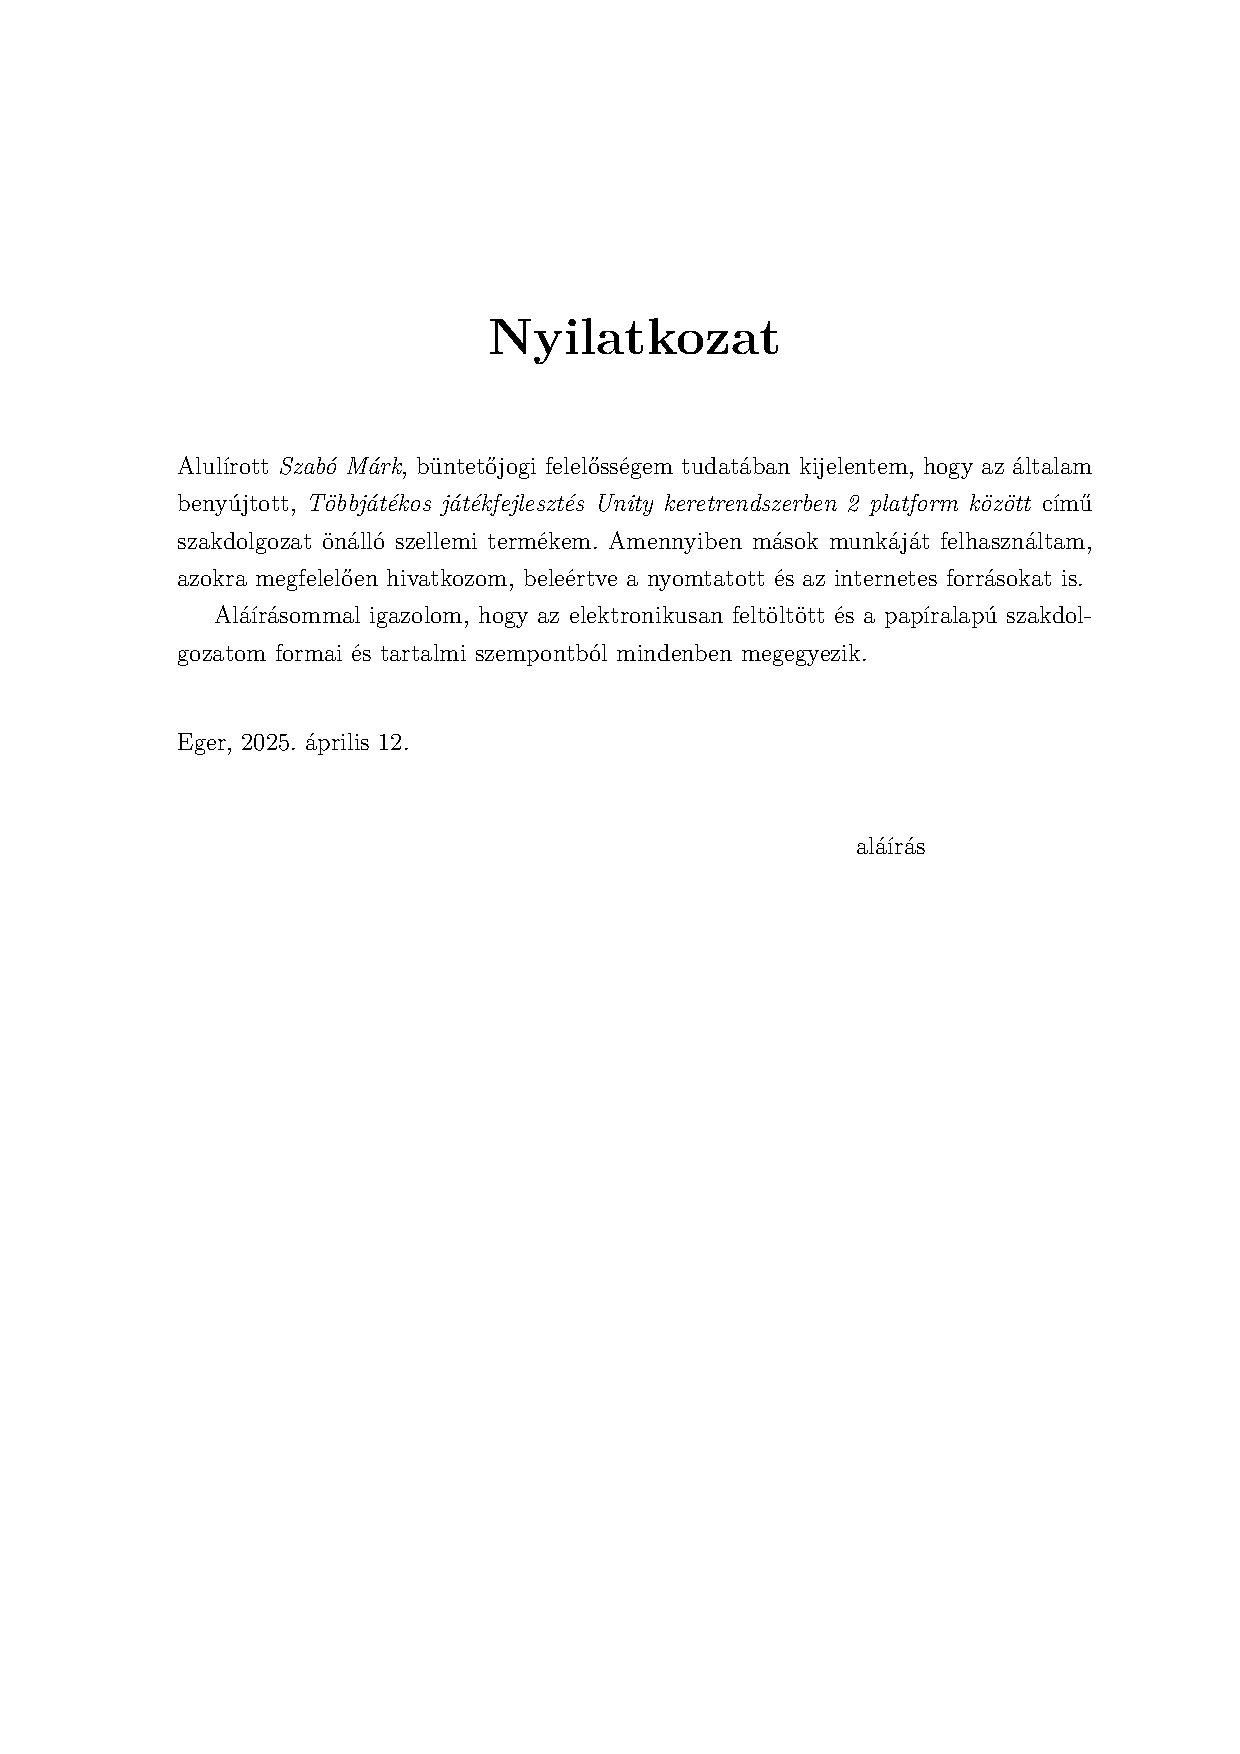
\includepdf{nyilatkozat/nyilatkozat.pdf}
\end{document}